\chapter{Conceitos Básicos}
\label{ch:2}
Neste capítulo discutiremos alguns conceitos básicos necessários ao entendimento da solução proposta. Abordaremos inicialmente sobre orientação a serviços e a componentes, apresentando as principais características de cada abordagem. 

Apresentaremos também a plataforma OSGi e o Framework iPOJO, que que são as tecnologias que formam o núcleo deste trabalho.

Em seguida, discutiremos sobre gerenciamento de recursos e serviços, sua importância no contexto de arquiteturas orientadas a serviços, e uma visão geral do ciclo de desenvolvimento PDCA. 

Por fim, apresentaremos uma visão geral de JMX, a tecnologia utilizada no trabalho para realizar o monitoramento dos recursos.

\section{Orientação a Serviços}
\label{sec:service}
Orientação a Serviços, surge como um novo paradigma de desenvolvimento de aplicações distribuídas, promovendo reuso, baixo acoplamento e interoperabilidade, através do conceito de serviços como unidades que representam funcionalidades da aplicação~\cite{erl2008soa}~\cite{cervantes2005technical}. 

Assim, na orientação a serviços, as capacidades dos serviços são definidas através de uma descrição do serviço (\textit{Service Description}), e a partir dessa descrição, provedores de serviço são descobertos por consumidores estabelecendo um contrato de serviço entre as partes. 

Deste modo, no mundo de serviços, temos diversas implementações distintas para um mesmo serviço, e o consumidor não está vinculado a nenhuma delas, podendo substituir o serviço consumido de acordo com suas necessidades, através da definição de novos contratos de serviço com base nessas descrições~\cite{cervantes2005technical}.

\subsection{\textit{Service Oriented Architecture}}
Alinhado a essas ideias, temos em SOA, um modelo de arquitetura baseada em serviços com suporte a descoberta dinâmica de serviços. O modelo arquitetural de SOA baseia-se nos 3 elementos fundamentais da orientação a serviços.

\begin{itemize}
 \item \textbf{Provedor de Serviços} (\textit{Service Provider})
 \item \textbf{Consumidor de Serviços} (\textit{Service Requestor})
 \item \textbf{Registro de Serviços} (\textit{Service Registry})
\end{itemize}

A interação destes elementos compões o triângulo tradicional do modelo, ver Figura \ref{fig:soatriangle}. 

A interação dos elementos é relativamente simples. Provedores de serviço publicam suas capacidades através de \textit{Service Descriptions} no registro de serviços.
O consumidor do serviço executa consultas a um determinado serviço, com base em sua descrição, através do registro. Caso exista um provedor que atenda as necessidades do consumidor, então o registro devolverá uma referência do provedor do serviço ao consumidor, possibilitando a realização do \textit{binding} entre eles. 

Então, o provedor disponibiliza um objeto que implementa a interface do serviço e representa o objeto remoto, em tempo de execução (\textit{Servant}~\cite{volter2005remoting}), finalizando a interação com o provedor. 

Quando a interação entre o consumidor e o \textit{servant} é finalizada, o mesmo é liberado para utilização em alguma outra requisição ou simplesmente destruído.

Nesse contexto, o consumidor não tem conhecimento de como o serviço é implementado, onde o mesmo se localiza, nem mesmo se o \textit{servant}, pelo qual ele tem acesso ao serviço, é o mesmo a cada invocação. Esse grau de transparência provê um grande potencial de dinamismo e reuso, que são duas das principais características de arquiteturas orientadas a serviços~\cite{davis2009open}.


\section{Orientação a Componentes}
\label{sec:component}
Segundo Szyperski ~\cite{szyperski2002component}, "Componentes de software são unidades binárias de produção, aquisição e implantação independente, que interagem formando sistemas".

Além disso, componentes definem interfaces e dependências através de um modelo de componente. Esses modelos, assim como classes da orientação a objetos, descrevem as características do modelo, ver \ref{sub:elements}.

A orientação a componentes também define o conceito de \textit{containers}, que gerenciam o ciclo de vida e encapsulam os componentes, intermediando sua interação com o mundo externo.

Um componente possui 3 propriedades características:

\begin{enumerate}
\item \textbf{Pode ser implantado de forma independente}

Diz respeito a implantação independente de ambiente ou de outros componentes.

\item \textbf{Não deve possui estado observável}

Diz respeito as instâncias de componentes, que não devem ser distinguíveis entre si, ou seja, não há o conceito de estado observável presente na orientação a objetos. Terceiros não conseguem diferenciar cópias de um componente.

\item \textbf{Unidade de composição com terceiros}

Essa propriedade traz consigo algumas características semelhantes as da orientação a serviços, uma vez que, para a realização de uma composição, o componente deve ser coeso, auto-contido e possuir interfaces bem definidas. 
Um componente pode ser visto como uma caixa preta, que encapsula detalhes de sua implementação e interage com o mundo externo através de sua(s) interface(s).
\end{enumerate}

Essas propriedades são realizadas por 3 elementos distintos que são base da orientação a componentes.

\subsection{\textit{Component Elements}}
\label{sub:elements}

\subsubsection{Modelo de Componente}
O conceito de modelo de componente é, de certa forma, similar ao conceito de classe na orientação a objetos~\cite{cervantes2005technical}. Ele abstrai e descreve as características dos componentes (interfaces, propriedades, dependências) e pode definir mecanismos pelos quais estes são implantados.

\subsubsection{Instância de Componente}
Uma instância de componente, retomando nossa analogia a orientação a objetos, é um elemento que representa uma entidade "física" do modelo. Diferente do modelo, uma instância de componente possui estado e pode fazer parte de composições~\cite{cervantes2005technical}~\cite{szyperski2002component}.

\subsubsection{Pacote de Componente}
Um pacote de componente pode ser definido como um componente pronto para ser implantado, ou seja, um componente auto-contido que possui todas as suas dependências resolvidas de maneira a prover suas funcionalidades de forma independente~\cite{cervantes2005technical}.

\subsection{\textit{Deployment Descriptors}}
Outro elemento importante no mundo de componetes, é o chamado \textit{Deployment Descriptior}, que é um arquivo de configuração que descreve um conjunto de propriedades que definem como o componente será implantado na plataforma~\cite{deploy}~\cite{deployoasis}. 

Geralmente essas propriedades são descritas em documentos XML~\cite{xml} devido a sua natureza semi-estruturada, representatividade e a facilidade de entendimento e escrita. Além de ser um padrão W3C ~\cite{w3c} amplamente utilizado atualmente.

\section{OSGi}
\label{sec:osgi}

Para iniciarmos uma introdução sobre OSGi, não podemos deixar de falar da \textit{OSGi Alliance}, um consórcio formado por grandes empresas que lideram vários segmentos do ramo de TI, cuja principal missão é criar um middleware universal para o desenvolvimento de aplicações modulares na plataforma Java~\cite{osgiorg}.

Java fornece a portabilidade necessária para suportar aplicativos em diferentes plataformas, porém, não dá suporte explícito à construção de sistemas modulares~\cite{hall2010osgi}. A plataforma OSGi provê um conjunto de especificações permitindo que aplicações sejam construídas de maneira colaborativa a partir de pequenos componentes reutilizáveis ~\cite{osgiorg}, simplificando o desenvolvimento e a manutenção do código~\cite{hall2010osgi}.

O principal componente da especificação OSGi é o Framework OSGi, ele fornece um ambiente padronizado onde as aplicações, denominadas \textit{bundles}, podem, em tempo de execução,  ser instaladas, desinstaladas, ativadas ou desativadas local ou remotamente.


\subsection{Arquitetura}

A arquitetura do OSGi define um conjunto de camadas, vistas na Figura \ref{fig:arch_osgi}. 

Iremos nos concentrar nas principais camadas do framework, apresentando-as nas próximas seções.

\begin{figure}[htp]
\centering
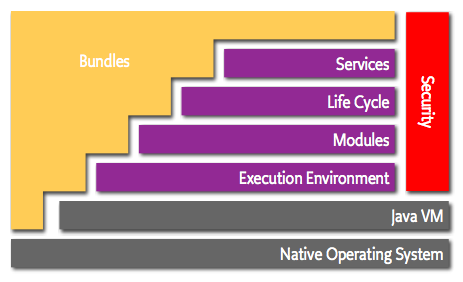
\includegraphics[width=9cm]{chapters/chapter2/arch-osgi.png}
\caption[Arquitetura OSGi]{Arquitetura OSGi~\cite{osgiorg}.}
\label{fig:arch_osgi}
\end{figure}


\subsubsection{\textit{Module Layer}}
Define o conceitos de módulos, providos através dos \textit{Bundles}. Um \textit{bundle} é nada mais que um arquivo JAR com um conjunto de metadados definidos em um \textit{Manifest}. De fato, a figura do \textit{bundle} é extremamente simples, porém, ao mesmo tempo poderosa, uma vez que, diferente de um simples arquivo JAR, um \textit{bundle} define um módulo lógico que pode ser combinado para a composição de uma aplicação~\cite{hall2010osgi}.

Além disso, ~\textit{bundles} podem declarar explicitamente dependências externas e pacotes exportados, ampliando o mecanismo de controle de acesso padrão de Java. Essa capacidades de declarar explicitamente pacotes importados e exportados, traz um grande benefício ao desenvolvedor, uma vez que, o próprio framework OSGi fica responsável por gerenciar e verificar a automaticamente consistência da aplicação, através do processo chamado de \textit{bundle resolution}~\cite{hall2010osgi}~\cite{osgiorg}.

\subsubsection{\textit{Lifecycle Layer}}
Controla o ciclo de vida dos \textit{bundles}, definindo como os mesmos são dinamicamente instalados e gerenciados. 

Também define como os \textit{bundles} obtem acesso ao \textit{bundle context}, controlando a interação dos mesmos com o framework.

É nesse contexto que temos a figura do ativador responsável por inicializar/parar o bundle, provido através da interface \textit{BundleActivator}, semelhante ao \textit{main} de um programa Java.

\subsubsection{\textit{Service Layer}}
Incorpora características de SOA no OSGi, com as figuras do registro, provedor e consumidor de serviço, visto na Seção \ref{sec:service}. 

Ela expande o dinamismo provido pelos textit{bundles} na camada de ciclo de vida, combinando este ao dinamismo provido por arquiteturas baseadas em serviço, onde serviços podem aparecer ou desaparecer a qualquer momento~\cite{hall2010osgi}.

\subsection{iPOJO}
\label{subsec:ipojo}
Outra tecnologia importante para a compreensão deste trabalho, é o framework iPOJO~\cite{ipojo}.

iPOJO implementa um modelo componentes orientados a serviço, que tem como principal objetivo simplificar o desenvolvimento de aplicações OSGi. Utiliza o conceito de POJO (\textit{Plain Old Java Objects}) para definir componentes, onde um POJO é basicamente um objeto java simples, que não possui nenhuma dependência do ambiente de execução.
	
No iPOJO, os diversos POJO's são encapsulados em \textit{containers}, responsáveis pelo gerenciamento das interações entre o POJO e o mundo externo ao \textit{container} e podem ser extendidos através da utilização de \textit{handlers}~\cite{ipojo}.

\begin{figure}[htp]
\centering
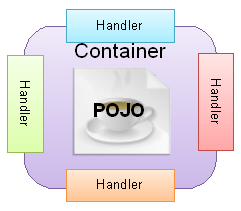
\includegraphics[width=5cm]{chapters/chapter2/ipojo-handlers.png}
\caption[Handlers Ipojo]{Handlers iPOJO~\cite{ipojo}.}
\label{fig:arch_osgi}
\end{figure}

A idéia por traz do iPOJO se baseia nos conceitos de orientação a componentes, onde temos, além da figura do \textit{container}, a visão de modelo e instância de componente. 

No iPOJO, o modelo de componente, chamado de \textit{component type}, especifica: um conjunto de propriedades do componente; sua classe de implementação e políticas de criação de instâncias. Onde cada instância herda todas as características do \textit{component type} e pode ter seu próprio conjunto de propriedade~\cite{ipojo}.

O iPOJO abstrai o uso de OSGi através do conceito de containers que controlam o acesso e gerenciam o ciclo de vida do POJO, e de \textit{handlers} ``plugados'' aos containers extendendo suas capacidades.


\section{Ciclo PDCA}
\label{sec:pdca}
O ciclo PDCA (\textit{\textbf{P}lain \textbf{C}heck \textbf{D}o \textbf{A}ct}), ou ciclo de  Demming, é um ciclo de desenvolvimento e gestão de processos com foco na melhoria contínua proposto por Walter A. Shewhart~\cite{shewhart} e amplamente difundido por W. Edward Deming~\cite{deming}, inicialmente utilizado-o na implementação de um sistema de qualidade na indústria japonesa ~\cite{fabio2003}.

O ciclo é dividido em 4 etapas, ver Figura \ref{fig:pdca}, que visam garantir o alcance de metas pré-estabelecidas, através da utilização de informações como fator chave na tomada de decisões.

É aplicável a diversas atividades de gestão, incluindo o gerenciamento de performance~\cite{pdcacont}. É um método eficaz de controle de atividades relacionadas a melhorias e compartilha dos conceitos de gerencia de redes e recursos em geral, a medida que, a tomada de decisão é fortemente influenciada pelas informações coletadas.


\begin{figure}[htp]
\centering
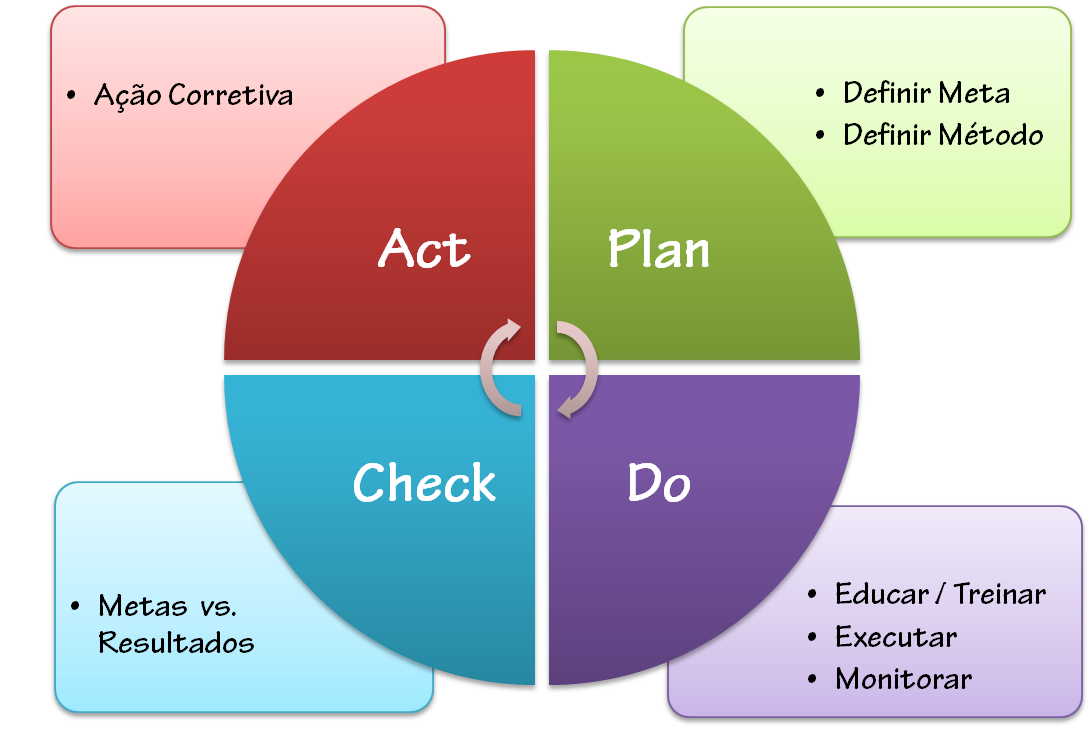
\includegraphics[width=7.5cm]{chapters/chapter2/pdca_cycle.png}
\caption[Ciclo PDCA]{Ciclo PDCA de Desenvolvimento com Foco na Melhoria Contínua.}
\label{fig:pdca}
\end{figure}


\subsection{Etapas}
\label{pdca:phases}
\subsubsection{\textit{Plan} - Planejar}
A fase de planejamento consiste no estabelecimento de metas e objetivos com base nas políticas adotadas pela organização~\cite{pdcacont}. Nesta etapa é de extrema importância a análise de informações para a identificação e o entendimento do problema a ser resolvido.

É a fase mais importante do processo, uma vez que, um planejamento bem elaborado reflete no resultado como um todo. Evitando falhas e perda de tempo em fases futuras~\cite{fabio2003}~\cite{pdcacont}.

Tem como resultado a elaboração de um plano de ação, que define os métodos necessários para atingir as metas estabelecidas.

\subsubsection{\textit{Do} - Executar}
É a fase de execução do plano de ação e coleta dos dados relacionados, para posterior análise~\cite{pdcacont}.

Nesta etapa é importante que a execução seja coerente com o plano de ação definido na fase anterior, uma vez que, enquanto a fase anterior busca maior eficácia e coesão, a fase de execução é voltada à eficiência do processo.

\subsubsection{\textit{Check} - Verificar}
É fase de verificação dos resultados obtidos da execução realizada na fase anterior. Com base nas metas e estratégias definidas na fase de planejamento em conjunto com os dados monitorados na fase de execução, a etapa de verificação foca na análise sistemática dos dados monitorados afim de verificar a efetividade das ações tomadas~\cite{pdcacont}.

A diferença entre o desejável, o planejamento, e o resultado alcançado constitui um problema a ser resolvido.

\subsubsection{\textit{Act} - Agir}
Nesta fase são realizadas as ações corretivas, com base na análise do resultados da fase anterior. Essas ações tem o intuito de evitar que o problema verificado na etapa anterior volte a acontecer~\cite{pdcacont}. Também estão definidas no plano de ação e além de buscar corrigir problemas, podem estar envolvidas na busca por melhoria contínua do processo~\cite{pdcaknow}.

\paragraph{}
A aplicação dessas etapas resulta no aprendizado do processo, o que repercute na tomada de decisão, uma vez que, utiliza de informações relevantes extraídas da execução do processo.

\section{JMX}
\textit{Java Management Extensions} (JMX) é uma API que fornece uma maneira simples e padrão de gestão e monitoramento de recursos para a plataforma Java. Estes recursos podem ser aplicações, dispositivos, serviços ou a própria JVM (\textit{Java Virtual Machine}). São instrumentados por um ou mais \textit{Managed Beans}, ou simplesmente MBeans, responsáveis por adquirir, manipular ou enviar informações acerca destes recursos~\cite{lindfors2002jmx}.

Essa tecnologia foi desenvolvida através do JCP (\textit{Java Community Process}), em duas JSRs (\textit{Java Specification Request}) distintas. A JSR 3, \textit{Java Management Extensions Instrumentation and Agent Specification} e a JSR 160, \textit{Java Management Extensions Remote API}, ver Seção \ref{subsec:arch}.

JCP é o processo de desenvolvimento padrão de novas especificações para a plataforma Java, as chamadas JRSs. JSRs são documentos que descrevem as especificações e tecnologias propostas à plataforma.

A especificação de JMX define, além da arquitetura, padrões de projeto, API's e um conjunto de serviços de gerenciamento e monitoramento. Possibilitando o desenvolvimento de aplicações gerenciáveis local ou remotamente através do processo de instrumentação, onde atributos, configurações e capacidades da aplicação são expostos. Aumentando a robustez e extensibilidade da aplicação, uma vez que, é possível construir soluções de gerenciamento inteligentes, interoperáveis e independentes da infra-estrutura de gestão~\cite{jmx}.

\subsection{Arquitetura}
\label{subsec:arch}
A arquitetura JMX é definida em três níveis, ver Figura \ref{fig:arch_jmx}:

\begin{itemize}
 \item Nível de Instrumentação;
 \item Nível de Agente;
 \item Nível de Gerenciamento.
\end{itemize}

Como foi dito anteriormente, JMX foi definida segundo duas JSRs , JSR 3 e JSR 160. Os dois primeiros níveis da arquitetura (Instrumentação e Agente) foram definidos na JSR 3, enquanto o Nível de Gerenciamento foi definido na JSR 160. Isso mostra, de certa forma, o potencial de extensibilidade da tecnologia.

\begin{figure}[htp]
\centering
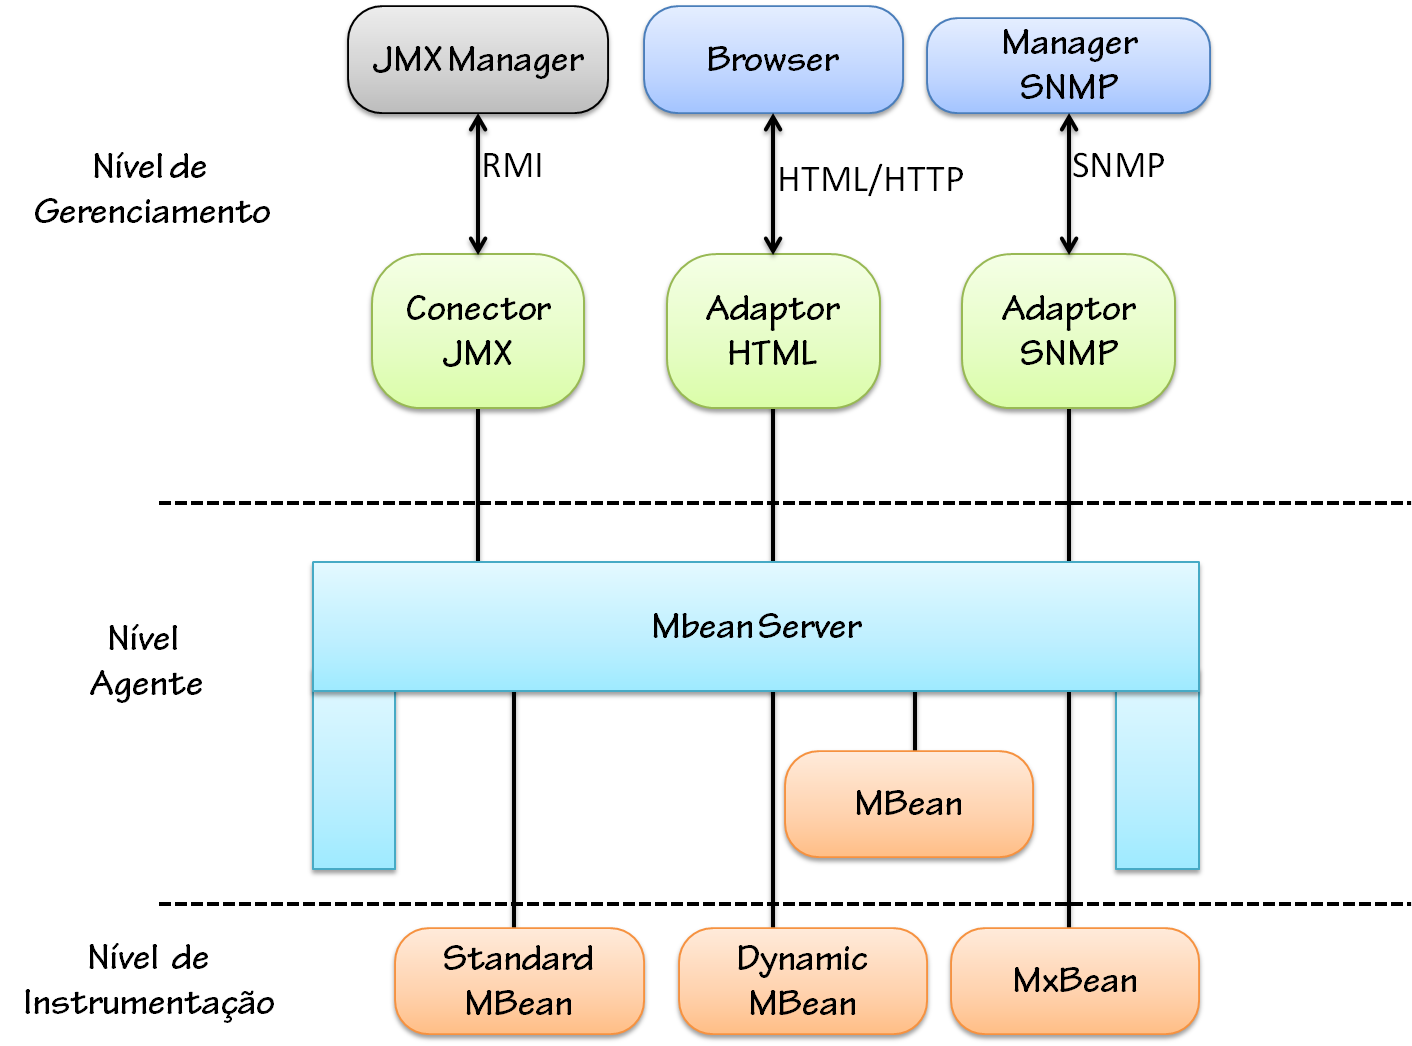
\includegraphics[width=12cm]{chapters/chapter2/arch_jmx.png}
\caption[Arquitetura JMX]{Arquitetura JMX.}
\label{fig:arch_jmx}
\end{figure}

\subsubsection{Nível de Instrumentação}
O nível de instrumentação é responsável por expor as funcionalidades e configurações das aplicações através da criação e registro de MBeans~\cite{jmx}. Estes MBeans coletam e manipulam informações dos recursos gerenciáveis, repassando-as aos agentes JMX do nível superior.

Exitem diferentes tipos de MBeans em JMX. Nas próximas seções descreveremos alguns dos mais importantes.

\paragraph{Standard MBean:}
\label{para:stardardmbean}
São os tipos mais simples de \textit{Managed Bean}. Interagem com os recursos gerenciáveis através da definição de uma interface de gerenciamento, que descreve os atributos e operações do MBean. Estas interfaces são definidas explicitamente e os atributos e métodos descobertos por meio de reflexão. Além disso, seguem a convenção do nome da classe acrescido do prefixo \verb MBean  e todos os seus atributos são acessados por métodos \textit{getters} e \textit{setters}. \textit{Standard Mbeans} possuem uma limitação quanto aos tipos de dados que podem ser utilizados, não permitindo o uso de tipos complexos definidos pelo usuário~\cite{mxbeans}.

Uma limitação da arquitetura JMX é que, não é permitido a implementação de duas interfaces de gerenciamento para a mesma MBean. Mesmo através de herança visando evitar a implementação explícita de duas interfaces, o agente JMX sempre irá utilizar a interface de gerenciamento mais próxima da classe. Uma alternativa a esse problema é estender a interface de gerenciamento.

\paragraph{MxBean:}
\label{para:mxbean}
Mxbean é uma versão melhorada do \textit{Standard MBean}, ele traz uma solução ao problema relacionado ao conjunto limitados de tipos de dados utilizáveis pela MBean comum, visto no parágrafo \ref{para:stardardmbean}.

Ele provê suporte à utilização de tipos de dados complexos, para representação de atributos do MBean, através de mapeamentos de tipos complexos para um tipo padrão \verb CompositeDataSupport ~\cite{mxbeans}.

A especificação de Mxbeans está presente na JSR 174 e este foi incluído na versão 6 de Java. Sendo assim, só pode ser executado nas versões superiores a J2SE 5.0~\cite{mxbeans}.

\paragraph{Dynamic MBean:}
\label{para:dynamicmbean}
\textit{Dynamic MBeans} se diferenciam de \textit{Standard MBeans} pelo fato de que estes descrevem seus atributos e operações através de uma interface genérica. Assim, as propriedades do MBean são descobertas em tempo de execução, já que, através dessa interface, os agentes JMX obtém a descrição da MBean por meio da classe \verb MBeanInfo ~\cite{jmx}. 

O diferencial é que no caso das \textit{Standard MBeans}, os metadados que descrevem a interface são obtidos por meio de reflexão, e na \textit{Dynamic MBean}, as classes de metadados são construídos por elas mesmas em tempo de execução.

Desde modo, o acesso ao atributos e operações em MBeans dinâmicas não é realizado diretamente, mas sim por meio de métodos genéricos, semelhante ao mecanismo utilizado pelo padrão de projeto \textit{Requestor}~\cite{volter2005remoting}. Esse método de acesso é ilustrado na figura \ref{fig:requestjmx}.

\begin{figure}[htp]
\centering
\subfloat[Invocação de Operação na MBean]{
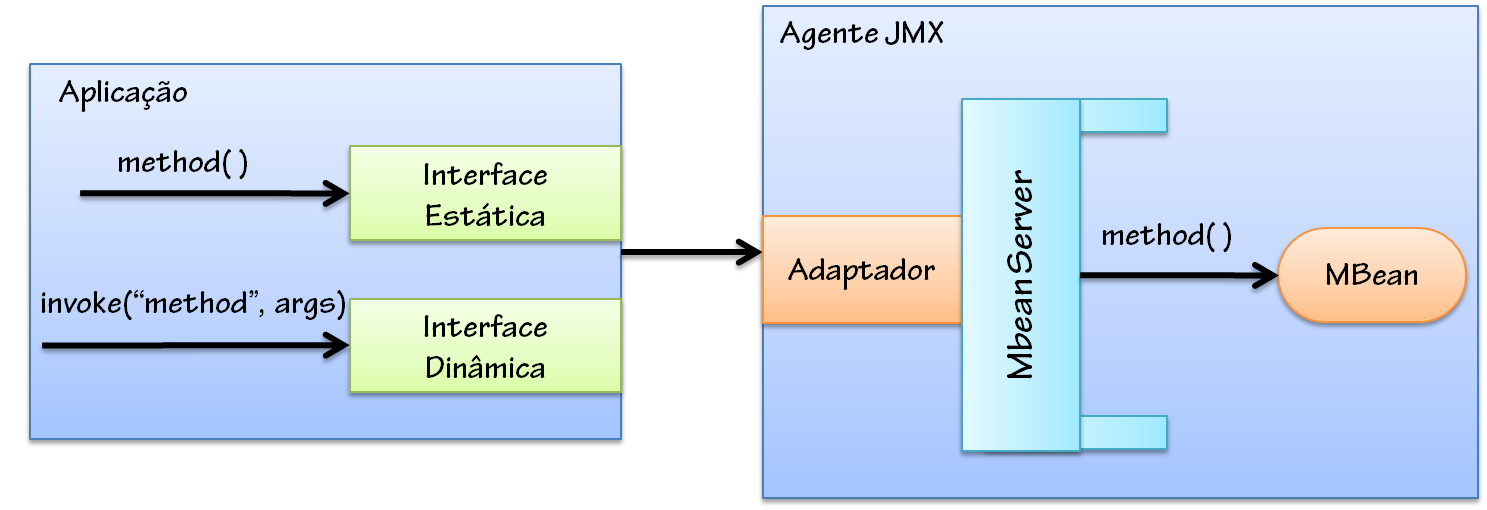
\includegraphics[width=13cm]{chapters/chapter2/invoke.png}
}
\\
\subfloat[Acesso a atributo na MBean]{
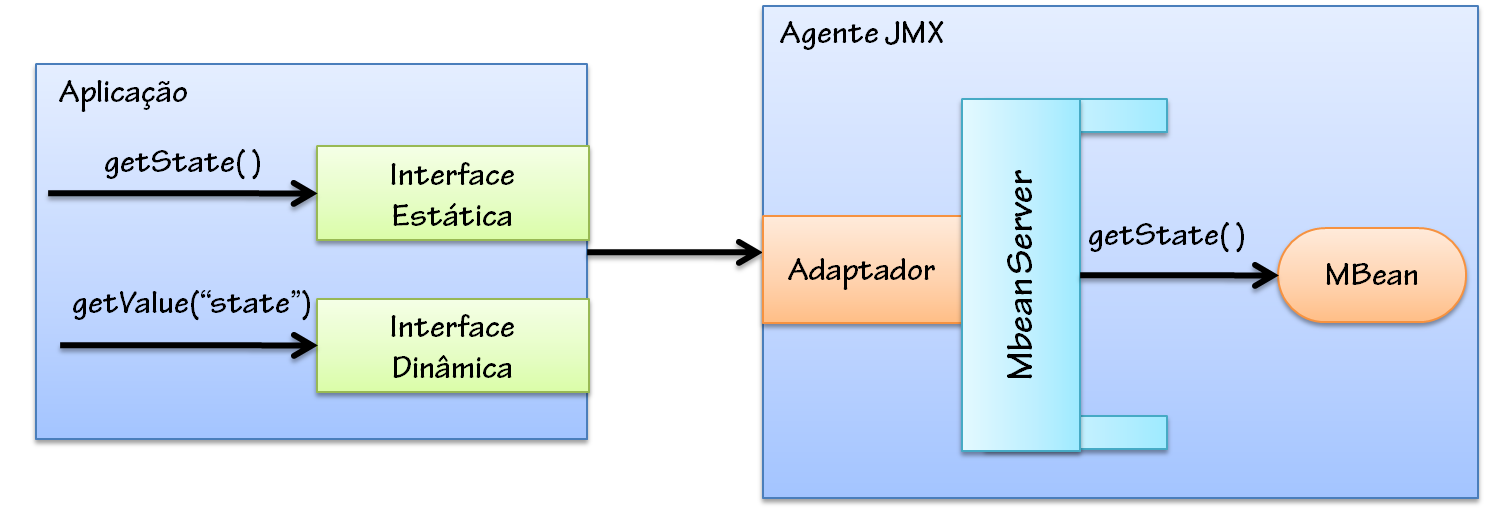
\includegraphics[width=13cm]{chapters/chapter2/getValue.png}
}
\caption{Acesso a atributos e operações da MBean.}
\label{fig:requestjmx}
\end{figure}

Exitem outros tipos de MBeans dinâmicas, como Model MBean, Open MBean e AbtractDynamicMBean que basicamente adicionam novas features à Dynamic MBean tradicional. Não entraremos em detalhes pois está fora do escopo deste trabalho.

\subsubsection{Nível Agente}
O nível agente é responsável por gerenciar todas as Mbeans e através delas controlar diretamente todos os recursos, tornando-os acessíveis a aplicativos de gerenciamento remoto.

A gerência das MBeans é provida através do principal componente do agente JMX, o MBean Server. Além disso, agentes JMX incluem um conjunto de serviços de gerenciamento de MBeans e pelo menos um adaptador de comunicações ou conector para permitir o acesso ao agente por aplicativos de gerenciamento~\cite{jmx}.

Basicamente, um agente JMX consiste em um MBean Server, um conjunto de serviços básicos de gerência e pelo menos um adaptador de comunicação ou conector JMX.

\paragraph{MBean Server:}
O MBean Server é o principal componente do nível agente. É o intermediário entre o sistema de gerenciamento e os objetos gerenciáveis (recursos), uma vez que, é responsabilidade do MBean Server registrar e manipular as MBeans~\cite{jmx}.

Para registrar uma MBean no servidor, além do próprio objeto MBean, é necessário que seja registrado junto a MBean um ObjectName que identifica unicamente aquela MBean no servidor. Além de identificar a MBean, ele permite a seleção de objetos a partir de mascaras no formato [domínio]:[par chave/valor]. \\
\verb org.meudominio:local=UFPE,nome=MBean \\

A manipulação de MBeans é feita através do MBean Server que provê um conjunto de operações comuns aos diferentes tipos de MBeans, uma vez que, os atributos e operações são descobertos através de classes de metadados comuns, ver parágrafo \ref{para:dynamicmbean}.

\subsubsection{Nível de Gerenciamento}
O nível de gerenciamento é o nível mais alto da arquitetura JMX, este define um mecanismo baseado em adaptadores e conectores que tornam os agente JMX acessíveis a aplicativos de gerenciamento remoto fora da JVM em que o agente encontra-se~\cite{jmx}.

Define, de certa forma, uma interface de acesso a agentes JMX para o mundo externo, através de protocolos proprietários ou existentes (\textit{e.g.} SNMP - \textit{Simple Network Manager Protocol}, um protocolo padrão para gerenciamento de componentes de rede)~\cite{douglas2005essential}.

Essa interface é garantida através de conectores e adaptadores que disponibilizam o acesos aos agentes JMX para diferentes tecnologia de gerenciamento.

A principal diferença entre conectores e adaptadores é que adaptadores surgem como uma solução de integração a sistemas que não dão suporte direto a JMX, por exemplo, sistemas de gerenciamento baseados em SNMP ou HTTP como Zabbix~\cite{zabbix} ou Nagios~\cite{nagios}, fornecendo uma visão de todos os MBeans através de um determinado protocolo. 

Já conectores, fornecem uma interface de gerenciamento remoto transparente e independente de protocolo~\cite{jmx}.


\subsection{Mecanismo Notificações}
Além dos três níveis de arquitetura, JMX provê um mecanismo de notificação que permite que aplicações ou MBeans recebam eventos ou notificações com informações sobre o estado dos recursos gerenciados, podendo gerar estatísticas ou mesmo processar eventos relacionados ao funcionamento dos recursos~\cite{lindfors2002jmx}.

O modelo de notificação JMX é semelhante ao mecanismo de notificações de java, que define \textit{object listers} (recebem as notificações) registados a MBean que envia as notificações \textit{(broadcaster MBeans)}. A \textit{broadcaster MBeans} envia eventos de notificação a todos os \textit{listeners} registrados~\cite{lindfors2002jmx}.

\subsubsection{Componentes do Mecanismo de Notificações}

O mecanismo de notificações JMX possui os seguintes componentes:

\begin{center}
\begin{table*}[h]
\begin{supertabular}[]{|l|l|}
\hline
\textbf{Componente} & \textbf{Descrição}\\\hline
Notification & Representa um tipo genérico de notificação\\\hline
NotificationListener & Interface que permite o recebimento de notificações\\\hline
\multirow{2}{*}{NotificationFilter} & Interface que permite a filtragem de notificações. Assim, apenas\\ 
& notificações relevantes ao Listener são recebidas\\\hline
\multirow{2}{*}{NotificationBroradcaster} & Interface que permite que notificações sejam enviadas aos\\
& listeners registrados \\\hline
\end{supertabular}
\caption{Componentes do Mecanismo de Notificação}
\end{table*}
\end{center}

\subsubsection{Modelo de Notificação JMX}
O modelo de notificações JMX segue os seguintes passos, demonstrados na Figura \ref{fig:notifyjmx}

\paragraph{Funcionamento} 
\begin{enumerate}
\item MBean consumidor registra-se através da interface \textit{NotificationBroadcaster}

\item MBean gerador emite uma notificação

\item A notificação é enviada aos MBeans registrados

\item O MBean consumidor recebe e filtra as notificações

\item As notificações não descartadas são tratadas
\end{enumerate}

\begin{figure}[htp]
\centering
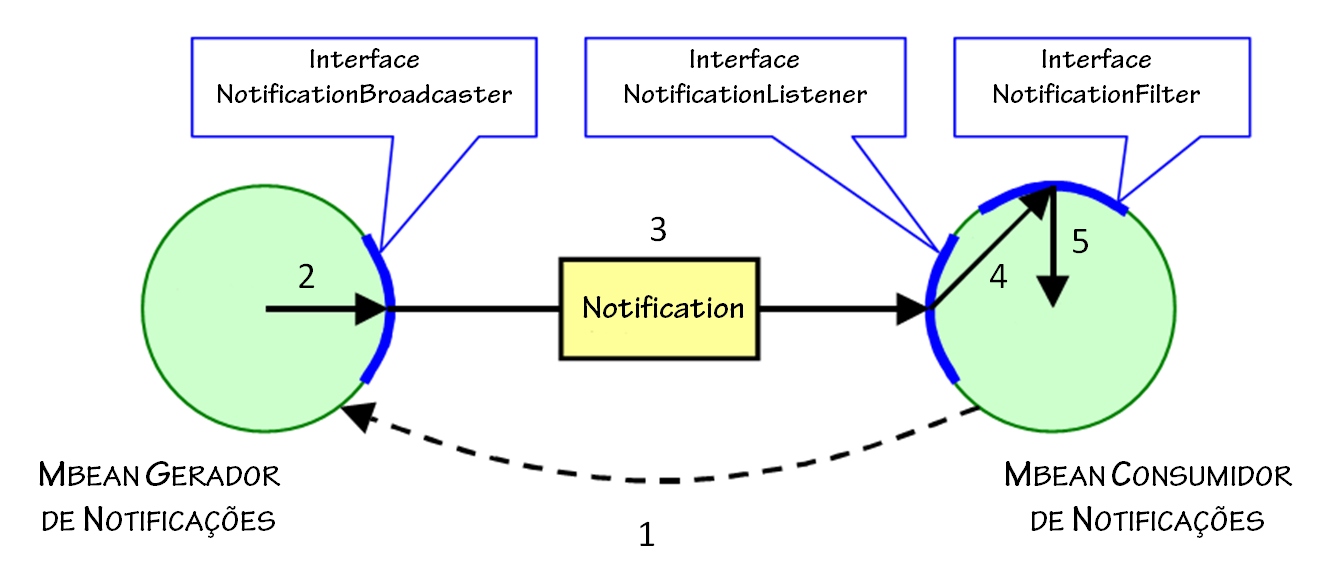
\includegraphics[width=13cm]{chapters/chapter2/notification_model.png}
\caption[Modelo de notificação JMX]{Modelo de notificação JMX~\cite{pericasgerencia}.}
\label{fig:notifyjmx}
\end{figure}

Assim, JMX surge como uma tecnologia de monitoramento e notificação flexível, dinâmica e extensível, sendo utilizada em diversas ferramentas comerciais (\textit{e.g. } JBoss Application Server - JBoss~\cite{jboss}, JOnAS Application Server - OW2 Consortium~\cite{jonas}, Tivoli Composite Application Manager - IBM~\cite{tivoli}). 

\section{Considerações Finais}
Assim, concluímos o capítulo que apresenta os conceitos essenciais ao entendimento dos próximos capítulos e do trabalho como um todo.

Apresentamos os paradigmas de orientação a serviços e componentes, assim como as plataforma OSGi e iPOJO, que são bases tecnológicas do mecanismo proposto. 

E demos uma visão geral do ciclo de desenvolvimento PDCA e da tecnologia de monitoramento de recursos utilizada neste trabalho, a tecnologia JMX.